%%%%%%%%%%%%%%%%%%%%%%%%%%%%%%%%%%%%%%%%%%%%%%%%%%%%%%%%%
%                                                       %
%  情報処理学会全国大会投稿論文用テンプレートファイル   %
%                   for ips.sty ver2.1                  %
%                                                       %
%%%%%%%%%%%%%%%%%%%%%%%%%%%%%%%%%%%%%%%%%%%%%%%%%%%%%%%%%

%%% ver2.1 +
%%% edited by Jutori
%%% modified by Kenta

\documentclass[a4paper,9pt, twocolumn]{jarticle}
%\documentclass[a4paper,9pt,twocolumn]{ipsjpapers}
\usepackage{graphicx}
\usepackage{ips}
\usepackage{mediabb}
\usepackage{here}

\renewcommand{\baselinestretch}{0.87}   % 行間

\pagestyle{empty}
%%%%%%    TEXT START    %%%%%%
\begin{document}

%%%%%%%%%%%%%%%%%%%%%%%%%%% ヘッダ %%%%%%%%%%%%%%%%%%%%%%%%%%
\twocolumn[%
\begin{center}

%--------------------------------------------------------------
% 講演タイトル(2行にわたるときは\2jtitle{}{}{})
%--------------------------------------------------------------

\vspace{-3mm}
\2jtitle{}{独自ベクトル処理機能を備えたプロセッサ向け}{自動ベクトル化コンパイラの開発}

%--------------------------------------------------------------
% 日本語著者名
%--------------------------------------------------------------
% name{1}{***} : 所属1の氏名
% name{2}{***} : 所属2の氏名 のようにする.所属の引数は4まで
% 名前は絶対間違えないように

\begin{authors}
\name{1}{永池 晃太朗}
\name{2}{大津 金光}
\name{2}{横田 隆史}
\name{2}{小島 駿}
\end{authors}
%--------------------------------------------------------------
% 所属
%--------------------------------------------------------------
% aff{1}{***} : 所属1
% aff{2}{***} : 所属2 のようにする.所属の引数は4まで.

\begin{affiliation}
\aff{1}{宇都宮大学工学部情報工学科}
\aff{2}{宇都宮大学大学院地域創生科学研究科}
\end{affiliation}

%--------------------------------------------------------------
\end{center}
]%

%%%%%%%%%%%%%%%%%%%%%%%%    脚注   %%%%%%%%%%%%%%%%%%%%%%%%%%

%--------------------------------------------------------------
% 英文タイトル
%--------------------------------------------------------------

\etitle{Development of automatic vectorization compiler for processors with original vector processing function.}


%--------------------------------------------------------------
% 英語語著者名
%--------------------------------------------------------------
% ename{1}{***} : 所属1の氏名
% ename{2}{***} : 所属2の氏名 のようにする.

%\ename{1}{First Last, First Last and First Last}
%ename{2}を使う場合、所属1の人と2の人で改行されてしまうので、\enameをコメントアウトして以下のように直接書くのをおすすめ (空白は適宜調節のこと)
\footnotetext{%
    \hspace{-3mm}\raise1ex\hbox{{\scriptsize \dag}}Kotaro Nagaike,%
    \hspace{1.5mm}\raise1ex\hbox{{\scriptsize \dag\dag}}Kanemitsu Ootsu,%
    \hspace{1.5mm}\raise1ex\hbox{{\scriptsize \dag\dag}}Takashi Yokota,%
    \hspace{1.5mm}\raise1ex\hbox{{\scriptsize \dag\dag}}Shun Kojima,%
}
%ただし所属が3の場合は†††でなく‡となるので,\ddagと付けること
%\footnotetext{%
%    \hspace{-3mm}\raise1ex\hbox{{\scriptsize \dag}}First Last,%
%    \hspace{1.5mm}\raise1ex\hbox{{\scriptsize \dag}}First Last,%
%    \hspace{1.5mm}\raise1ex\hbox{{\scriptsize \dag\dag}}First Last,%
%    \hspace{1.5mm}\raise1ex\hbox{{\scriptsize \ddag}}First Last,%
%}
%\footnotetext{%
%    \hspace{-1mm}\raise1ex\hbox{{\scriptsize \dag\dag}}First Last and%
%    \hspace{1mm}\raise1ex\hbox{{\scriptsize \dag\dag}}First Last%
%}


%--------------------------------------------------------------
% 英語所属
%--------------------------------------------------------------
% eaff{1}{***} : 所属1
% eaff{2}{***} : 所属2 のようにする.所属の引数は4まで.
% ※日本語の所属と対応させること.
\eaff{1}{Department of Information Science, Faculty of Engineering, Utsunomiya University}
\eaff{2}{Graduate School of Regional Development and Creativity, Utsunomiya University}


%--------------------------------------------------------------
% 英語住所
%--------------------------------------------------------------



% 上マージン30mm 下25mm 横20mm 段組の間隔 7mm
% 印刷した後、自分で確認すること

%%%%%%%%%%%%%%%%%%%%%%%% ここから本文 %%%%%%%%%%%%%%%%%%%%%%%%%%
\section{はじめに}
%%intro.tex
FPGA (Field Programmable Gate Array)はユーザによって回路の再構成が可能なLSIであり,目的の処理をハードウェアとして実装可能なデバイスである.
近年FPGAの大容量化,高性能化によって大規模な回路が実現可能になった.これによりFPGAは自動運転を始めとする組込み分野での利用増加が期待されている.

FPGAを用いたハードウェア開発はHDL (Hardware Description Language)によるRTL(Register Transfer Level)設計が広く用いられている.RTLはFPGA上に構成する回路の信号の流れや制御構造を直接設計できる一方,動作検証やデバックが難しく,短期間で複雑な処理の開発は困難である\cite{bib:fpga}.
そのため,FPGAによる開発期間を短縮する方法として,専用ハードウェアとプロセッサを用いたソフトウェアによる処理を組み合わせる方法が考えられる.FPGA上のハードウェアリソースを用いて実装するプロセッサのことをソフトコアプロセッサという.
一般的に組込みシステムではそのコストやサイズ,消費電力などに制限があるためハードウェア資源に制約があることが多く,メモリバンド幅が限られることからメモリシステムの性能が高くないことが多い.メモリシステムの性能が低いと演算性能を高くしてもメモリアクセスに時間がかかり,結果としてシステム全体の性能はメモリシステムの性能によって左右される\cite{bib:2}.
そこで,ソフトコアプロセッサによる処理を考える.すべての処理を専用ハードウェア回路で行うのではなく,高い性能の求められない汎用的な処理についてはソフトコアプロセッサにて行うことにより開発する専用ハードウェア回路を削減でき,ソフトコアプロセッサの性能が向上して専用ハードウェア回路を削減しても求められた性能に達することができればハードウェアの開発コストを抑えることができる.

組込み分野ではAI技術に注目が集まっている.独立行政法人情報処理推進機構の調査によると,将来強化/新たに獲得したい技術として組込み/IoT関連企業の46\%がAI技術を挙げている\cite{bib:ipa}.

AI技術の応用としては画像認識などの画像処理が行われる.画像処理では画像を構成する画素に対して同じ処理を行うようなものが多い.このように複数のデータに対して同じ演算を行う処理については,単一命令で複数データの処理を行うSIMD (Single Instruction, Multiple Data)や,複数命令を並列に実行するMIMD (Multiple Instruction, Multiple Data)による並列処理で高速化が可能である\cite{bib:simd_mimd}.
MIMDは複数の制御を並列化することができるため,異なる処理を同時に実行するアプリケーションでは有効である.しかし,プロセッサに複数の制御ユニットをもたせる必要があるためSIMDと比較するとハードウェアのコストが大きくなる.一方SIMDは単一の制御ユニットで複数の演算ユニットを並列動作させるため制御ユニットのコストは低くなる.
データ並列処理では複数のデータに対して同じ処理を実行するためSIMDによって並列処理が可能である.

SIMDによる並列処理を行う場合,SIMD命令は1命令で演算するデータ数が決まっている.そのため演算性能を上げるために同時演算数を変更すると機械語コードを作り直す必要がある.異なる同時演算数でも同一の機械語コードを利用可能とするためには,機械語コードが同時演算数に依存しないスケーラブルなベクトル拡張が必要である.スケーラブルなベクトル拡張により機械語コードを変更することなく,必要に応じて容易に同時演算数を増やし高性能化することが可能となる.

スケーラブルなベクトル拡張を実現したものとしてオープンな命令セットアーキテクチャであるRISC-V\cite{bib:risc-v}をベクトル拡張したベクトル拡張付きRISC-V\cite{bib:kimura}が提案されている.ベクトル拡張付きRISC-Vは組込み機器に広く用いられているARMのベクトル拡張であるARM SVE (Scalable Vector Extension)\cite{bib:arm_sve}の命令セットを参考に組み込み向けにRISC-Vに拡張したものである.しかし,ベクトル拡張付きRISC-Vに対応したコンパイラが存在していない.そこで解決策としてベクトル拡張付きRISC-Vのベクトル命令のアセンブリコードを得るためのコンパイラの開発を検討した.

本論文では,第2章で現在のMIQSプロセッサについて述べる.第3章でベクトル拡張付きRISC-V命令の生成のために利用したコンパイラ基盤であるLLVM\cite{bib:llvm}について述べる.第4章で実際に命令生成のための実装について述べる.第5章では実際のソースコードからアセンブリコードの出力を行った結果について述べる.       % 同一ディレクトリのintro.texが読み込まれる
我々は機械語コードの変更なしに同時並列演算数を変更することができる,データ並列処理のためのスケーラブルなベクトル処理機能を備えたベクトル拡張付きRISC-Vを提案している\cite{bib:kimura}.

我々のベクトル拡張付きRISC-Vは,ARMのベクトル拡張であるARM SVE\cite{bib:arm_sve}を参考に組込み向けにRISC-V\cite{bib:risc-v}をベクトル拡張したものである.
これにより,機械語コードが同時演算数に依存しないスケーラブルなベクトル拡張を実現したが,ベクトル拡張に対応したコンパイラがない.アセンブリコードを生成はARM SVEのコンパイラによるARM SVEアセンブリコードを変換するといった手法を取っており,規模の大きいプログラム等の場合,アセンブリコードを得ることは容易ではない.

この問題に対して,解決策として既存のRISC-Vコンパイラに変更を加えることによって,ベクトル拡張付きRISC-Vアセンブリコードを得ることのできるコンパイラを開発するという手段を考えた.

コンパイラの開発はコンパイラ基盤であるLLVM[4]を用いて行う.コンパイラ基盤はコンパイラの機能がモジュール化されており,既存機能の再利用が可能になっている.そのため,コンパイラの開発の際にコンパイラ基盤を用いることによって独自部分のみの開発で済む.
前述した通りベクトル拡張付きRISC-VはRISC-Vを拡張したものであることから,LLVMのRISC-Vコンパイラとしての機能を再利用してコンパイラの開発を行う.

なお,使用するLLVMのバージョンは13.0.0である.

\section{ベクトル拡張付きRISC-V}

ベクトル拡張付きRISC-VはRISC-Vが有する4つのカスタム命令のためのオペコード領域のうち2つを利用しており,1つをベクトルロード,ストア命令,もう一方をベクトル演算命令とベクトル制御命令に使用している.
ベクトルロード,ストア命令のアドレスはベースとなるスカラレジスタの値にオフセットを加えることで計算する.オフセットはスカラレジスタ,ベクトルレジスタ,即値の3種類を指定できる.オフセットにベクトルレジスタを指定することでギャザー,スキャターによる非連続なロード,ストアを行う.

ベクトル演算命令は,プレディケートあり演算,プレディケートなし演算命令,即値による演算命令に分けられる.演算命令は,基本的な算術論理演算命令,乗除算命令,ベクトルレジスタの各要素の総和を求める命令やアドレス計算の際に用いるインデックスレジスタを生成する命令からなる.プレディケートあり演算命令ではプレディケートレジスタによるベクトルマスク制御を行う.

ベクトル制御命令はプレディケート演算命令とベクトル長操作命令に分けられる.プレディケート演算命令は,プレディケートレジスタ同士の論理演算を行う.ベクトル長操作命令は,スカラレジスタに対しベクトル長を足す等の命令がある.

以上の命令はARM SVEを参考にした命令であるが,その命令フォーマットはRISC-Vの命令形式に従ったものである.

レジスタの構成は,v0からv31のベクトルレジスタ,vp0からvp15のプレディケートレジスタ,ベクトル長レジスタ,x0からx31の汎用レジスタとなっている.
また,ベクトル拡張付きRISC-Vの基本命令はRV32Iの命令を組み込んでいる.

\section{LLVMコンパイラ基盤}
LLVMはC言語などのソースコードから中間表現であるLLVM IRに変換を行うフロントエンド,アセンブリコード生成を行うバックエンドからなる.本研究では独自命令生成のためにバックエンドに対して変更を加える.

\begin{figure}[t]
    \centering
        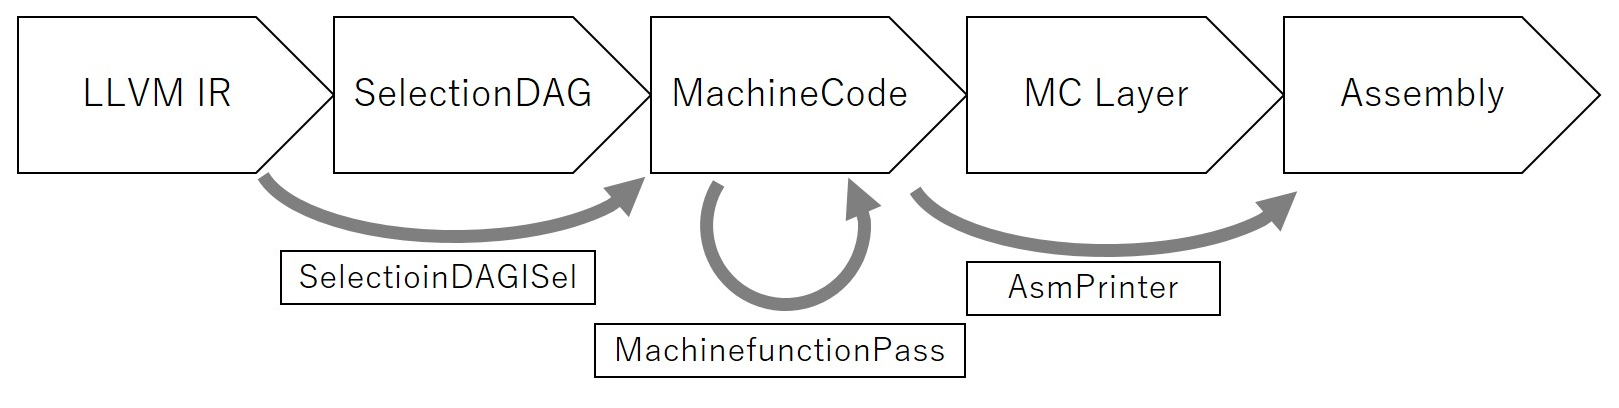
\includegraphics[scale=0.4]{backend.eps}
    \caption{コード生成の形式変換の流れ}
    \label{fig:backend}
\end{figure}

バックエンドにおけるコード生成について,処理の流れとパスを図1に示す.
SelectionDAGフェーズではSelectionDAGISelパスによってLLVM IRをDAG形式へと変換し,DAGのパターンマッチングによる命令の単純化,共通部分削除などの最適化,ターゲット命令への変換の順に行う.SelectionDAGISelは命令変換を行った後にMachineCode形式を出力する.
MachineCode形式はターゲットが使用する実際の命令を持った形式であり,MachinefunctionPassによってSSAベースの最適化を行い,命令への物理レジスタの割当を行う.レジスタの割当を行った後は非SSA形式となる.
MC LayerはAsmPrinterパスでアセンブリコード,オブジェクトコードを出力するための命令形式であり,関数などの構造がない.

以上のLLVMバックエンドでの処理はレジスタ情報,命令フォーマットや命令などのターゲット情報に従って行われる.
これらのターゲット情報はLLVMにおけるターゲット情報記述のためのドメイン固有言語であるTableGenによって行われる.

LLVMではRISC-VのV拡張用にTableGenによるベクトルレジスタ,ベクトル命令の定義が既に存在している.本研究ではベクトルレジスタはそのまま使用し,ベクトル命令については既存の定義に従った形式でベクトル拡張付きRISC-V命令の定義を行う.

また,ベクトル命令生成のための機能としてLLVMには自動ベクトル化機能が備わっている.フロントエンドにて入力ソースコードの繰り返しによる処理をベクトル化されたLLVM IRに変換を行う.
ベクトル化されたLLVM IRからパターンマッチングにより各ターゲットへのベクトル命令への変換などが行われる.RISC-VのV拡張用のパターンマッチングについても実装済みのものを再利用する.

\section{LLVMバックエンドにおける独自命令の生成機能の実装}

\begin{figure}[t]
    \centering
        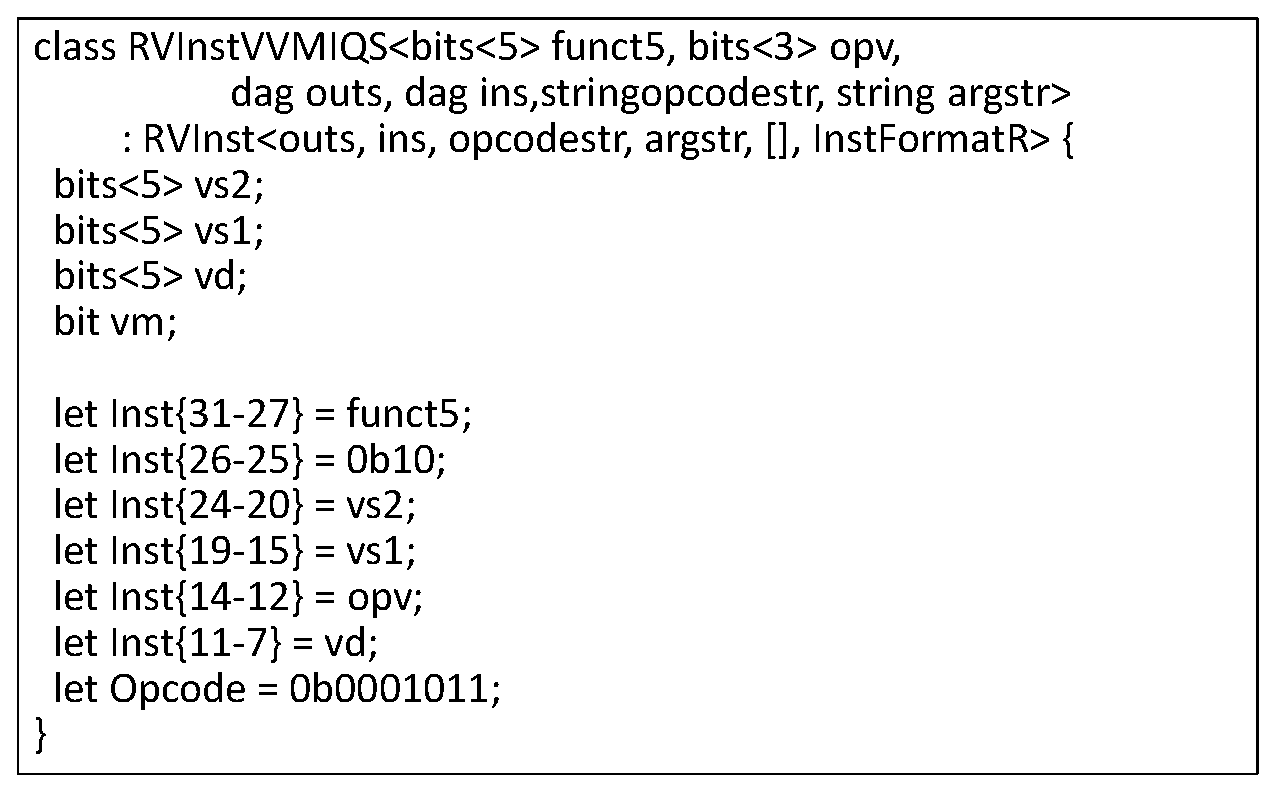
\includegraphics[scale=0.35]{RVInstVVMIQS.eps}
    \caption{命令フォーマットの定義}
    \label{fig:Instruciton_format}
\end{figure}

ベクトル拡張付きRISC-V命令の定義のために,図2のようなクラスを定義した.クラスRVInstVVMIQSは2つのベクトル要素を入力に持ち,ベクトル要素を出力する命令の命令フォーマットである.各命令フォーマットは32bitの命令フィールドを定義している基本クラスRVInstを継承する形で命令によって異なるフォーマットを定義する.

\begin{figure}[t]
    \centering
        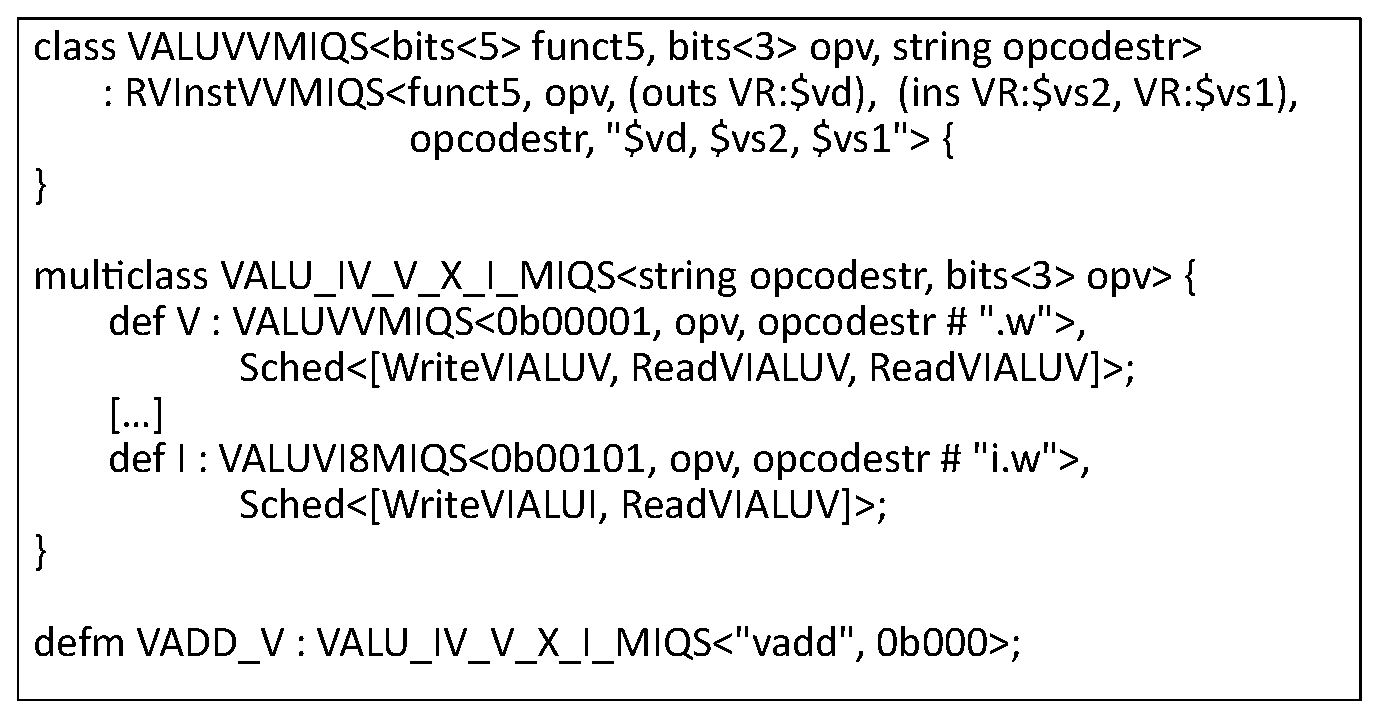
\includegraphics[scale=0.35]{Instruction.eps}
    \caption{命令の定義}
    \label{fig:Instruciton}
\end{figure}

命令の定義は命令フォーマットのクラスを継承し,エンコードの値やニーモニックを指定して行う.ベクトル拡張付きRISC-V命令の定義を図3に示す.図3のVALUVVMIQSクラスはベクトル算術演算用の命令定義であり,入力レジスタと出力レジスタの指定を行う.
また,図3にて命令のインスタンス化も行っており,ここで命令の文字列と命令選択に用いるための12-14ビットの値の指定を行っている.

現在ベクトル拡張付きRISC-Vのベクトル命令の内,ベクトル演算命令のプレディケートなし,即値による演算命令の実装が完了している.

\section{おわりに}
本研究では,自動でベクトル化された独自のベクトル拡張付きRISC-V命令アセンブリコードを得るためのLLVMバックエンドの実装を行った.

今後の課題として,未実装の命令生成の実現が挙げられる.
現在実装済みの命令は命令の定義等で実装が可能であったが,未実装の命令についてはレジスタの定義に加え,現在のベクトル化されたLLVM IRからの生成は困難であると考えられるためフロントエンドへの変更が必要と考える.

\renewcommand{\baselinestretch}{0.83}\selectfont
\subsection*{\small 謝辞}
\vspace{-0.5mm}
{\small 本研究は一部 JSPS 科研費 20K11726 の援助による.}
% 科研費IDや重点はその年によって記述が変わるのでよく確認すること
% 2015年時
% 調べ方:「 科研費 教授名」でぐぐる-> 研究課題番号


%
% ------ 参考文献 ------
%
\begin{thebibliography}{9}
\itemsep -1.7pt

\bibitem{bib:kimura}
{\small Yoshiki Kimura,et al:      % 丁寧
%{\small 氏名ほか:             % スペースが足りない場合
\newblock ``Proposal of Scalable Vector Instruc-tion Set for Embedded RISC-V Processor,''
\newblock Proc. 2019 Seventh International Symposium on Computing and Networking Workshops (CANDARW),
\newblock Vol.1,
\newblock pp.435-439,
\newblock 2019.}

\bibitem{bib:arm_sve}
{\small Nigel Stephens, et al:      % 丁寧
%{\small 氏名ほか:             % スペースが足りない場合
\newblock ``The ARM Scalable Vector Extension,''
\newblock IEEE Micro,
\newblock Vol.37,
\newblock No.2,
\newblock pp.26-39,
\newblock 2017.}

\bibitem{bib:risc-v}
{\small Andrew Waterman, Krste Asanovi:      % 丁寧
%{\small 氏名ほか:             % スペースが足りない場合
\newblock ``The RISC-V Instruction Set Manual Volume I: Unprivileged ISA,Document Version 2.2,''
\newblock 2017.}

\bibitem{bib:llvm}
{\small Chris Lattner, Vikram Adve:      % 丁寧
%{\small 氏名ほか:             % スペースが足りない場合
\newblock ``LLVM: A Compilation Frame-work for Lifelong Program Analysis Transformation,''
\newblock Proc. 2004 International Symposium on Code Generation and Optimization (CGO’04),
\newblock pp.75,
\newblock 2004.}

\end{thebibliography}

\end{document}

